\documentclass[a4paper,titlepage,openany,12pt]{book}
\usepackage{BackGround}
\usepackage{varwidth}
\usepackage{frontespizio}
\usepackage{qtree}


\makeindex

\begin{document}
\begin{frontespizio}
\Universita{Dell'insubria}
%\Logo{duck}
\Facolta{Informatica}
\Corso{Laboratorio A}
\Annoaccademico{2025--2026}
\Titolo{CineMax}
\Sottotitolo{Progetto di laboratorio A}
\Sottotitolo{manuale tecnico}
\Candidato[721086]{Francesco Ferrari}
\Candidato[768081]{Nithay Patricia Gomez Silva}
\Candidato[766922]{Pasquale Di Tuccio}
\Candidato[765700]{Luca Gabriel Chindris }

\end{frontespizio}


\chapter*{introduzione}


\tableofcontents

\chapter{Installazione}
In questo capitolo sono presentati i requisiti necessari all'installazione dell'applicazione e la modalità di installazione sui PC. \textbf{ATTENZIONE:} si segnala che questo programma è pensato per funzionare su sistemi Microsoft Windows, pertanto l'esecuzione su sistemi diversi non è garantita.

\section{Requisiti di sistema}

\section{Setup ambiente}

\section{Installazione programma} 

\chapter{Esecuzione ed uso}
In questo capitolo sono esposti i principali metodi che garantiscono il funzionamento dell'applicazione.
Viene anche discusso come è stato creato l'eseguibile e le modalità di setup e installazione dell'applicazione.

\section{Setup e lancio del programma}

\section{Classi e funzionalità}
In questa sezione sono descritte le parti fondamentali dell'applicazione, che ne garantiscono il funzionamento corretto;
Viene discussa la struttura e l'ereditatietà delle classi.

\subsection{Le classi}

\begin{figure}[!htbp]
\centering
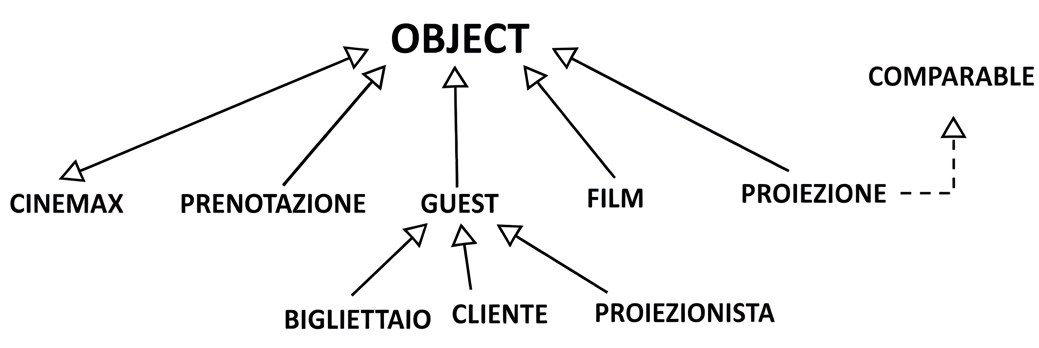
\includegraphics[scale=0.5]{IMGS/alberoclassi}
\caption{Albero dell'ereditarietà del progetto}
\end{figure}

In questa applicazione JAVA (package CineMaX) la classe Oblect è estesa direttamente dalle classi Film, Prenotazione, Proiezione (che implementa l'interfaccia Comparable),CineMaX e Guest. Le prime tre servono per creare oggetti di nome corrispondente: gli ogetti di tipo Film servono per costruire oggetti di tipo Proiezione, che rappresentano i film che è possibile inserire o modificare nel palinsesto, mentre il tipo Prenotazione rappresenta le prenotazioni effettuate da un cliente.
Infine CineMaX è la classe che contiene il metodo main e i metodi necessari alla registrazione e al login di un account utente (si veda la sezione \ref{subsubsec:CineMaX}).\\
La classe Guest ha tre sottoclassi dirette: Cliente, Proiezionista e Bigliettaio; Guest fornisce i metodi per effettuare la ricerca di una proiezione nel palinsesto (si veda la sezione \ref{subsubsec:Guest}), Cliente consente di effettuare,modificare o eliminare prenotazioni oltre alla ricerca di proiezioni (si veda la sezione \ref{subsubsec:Cliente}), Proiezionista consente di interagire col palinsesto inserendo, rimuovendo o modificando una proiezione (si veda la sezione \ref{subsubsec:Proiezionista}) e infine Bigliettaio consente di visualizzare e ricercare prenotazioni effettuate dai clienti (si veda la sezione \ref{subsubsec:Bigliettaio}).





\subsubsection{La classe Film}
La classe Film estende direttamente Object e serve unicamente per creare e operare su oggetti utilizzati nella costruzione di oggetti di tipo Proiezione, gli oggetti di tipo Film modellano il film da inserire nel palinsesto delle proiezioni e contengono le informazioni generali di un film, che sono:

\begin{center}
\begin{varwidth}{\textwidth}
\begin{itemize}
\item[•] \textbf{private String Titolo} 
\item[•] \textbf{private String Genere} 
\item[•] \textbf{private String Regista} 
\item[•] \textbf{private String Anno di pubblicazione} 
\item[•] \textbf{private String Durata}
\item[•] \textbf{private int Età}
\end{itemize}
\end{varwidth}
\end{center}

\begin{figure}[!htbp]
\centering
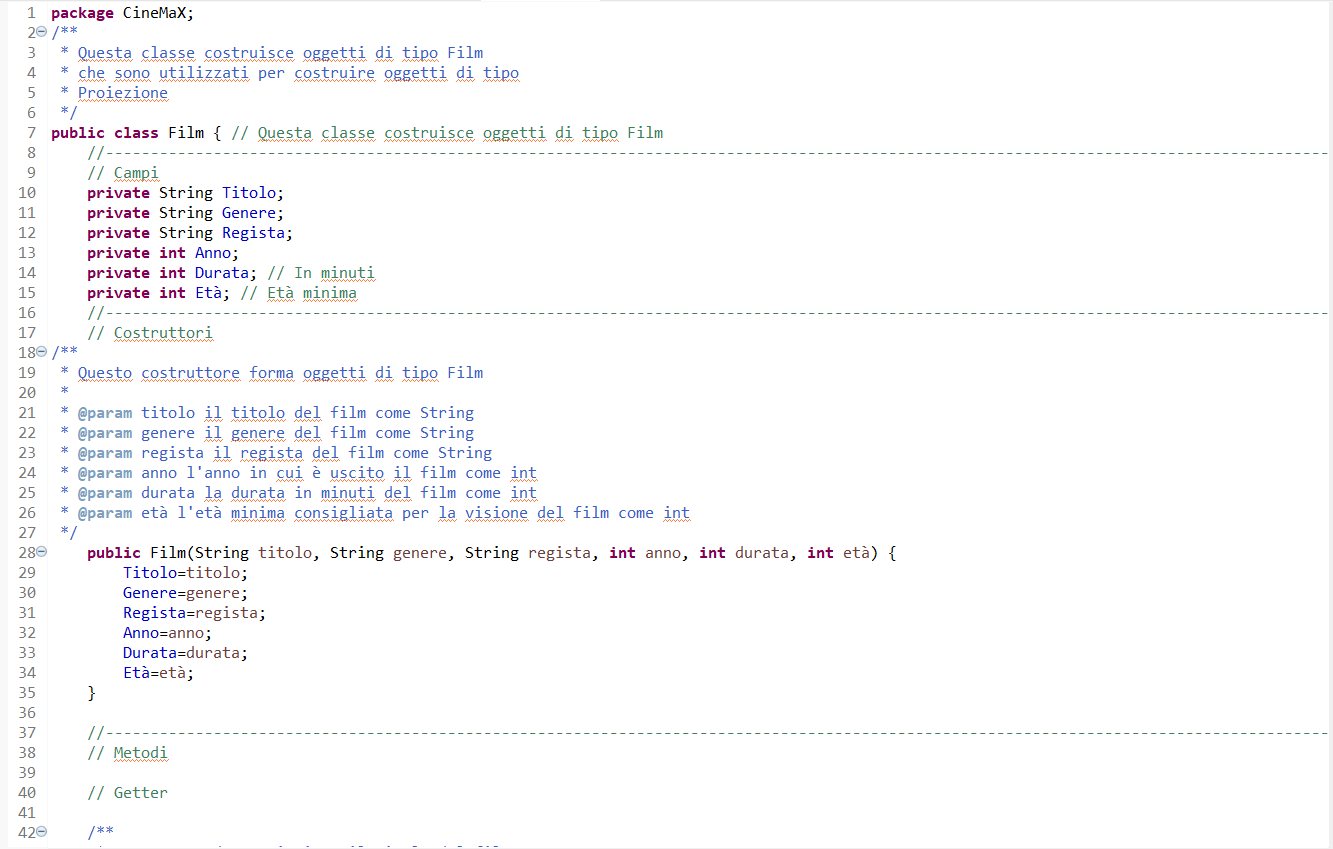
\includegraphics[scale=0.6]{IMGS/classefilm}
\caption{I campi e il costruttore della classe film}
\end{figure}

La classe contiene inoltre un costruttore, i metodi get e set per i campi e un metodo per stampare i campi mostrato in figura
 \ref{fig:stampacampi}.
\begin{figure}[!htbp]
\centering
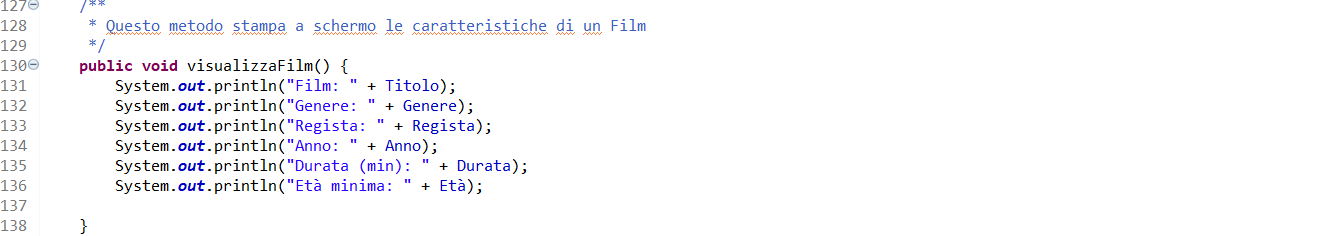
\includegraphics[scale=0.6]{IMGS/stampacampifilm}\label{fig:stampacampi}
\caption{Metodo che stampa le caratteristiche di un film}\label{fig:stampacampi}
\end{figure}

\subsubsection{La classe Proiezione}
La classe proiezione crea gli oggetti che modellano le proiezioni del palinsesto, questa classe estende direttamente la classe Object e implementa l'interfaccia Comparable<Proiezione> per consentire l'ordinamento cronologico automatico degli spettacoli in memoria. I suoi campi sono:

\begin{center}
\begin{varwidth}{\textwidth}
\begin{itemize}
\item[•] \textbf{private Film film} 
\item[•] \textbf{private LocalDateTime  dataOra}
\item[•]\textbf{private double PrezzoBiglietto} 
\item[•] \textbf{private int numeroPosti}
\item[•] \textbf{public static final int CAPIENZA\_ MASSIMA=200} 
\item[•] \textbf{private static final String FILE\_ PROIEZIONI}
\end{itemize}
\end{varwidth}
\end{center}

che rappresentano rispettivamente il film proiettato, la data e l'orario della proiezione in formato AAAA-MM-GG HH:MM:SS il prezzo del biglietto, il numero di posti prenotati, la capienza massima della sala del cinema e il percorso del file palinsesto proiezioni.csv.
Questa classe, oltre ai metodi get, set e al costruttore, contiene i metodi accessori della classe Proiezionista.

\begin{figure}[!htbp]
\centering
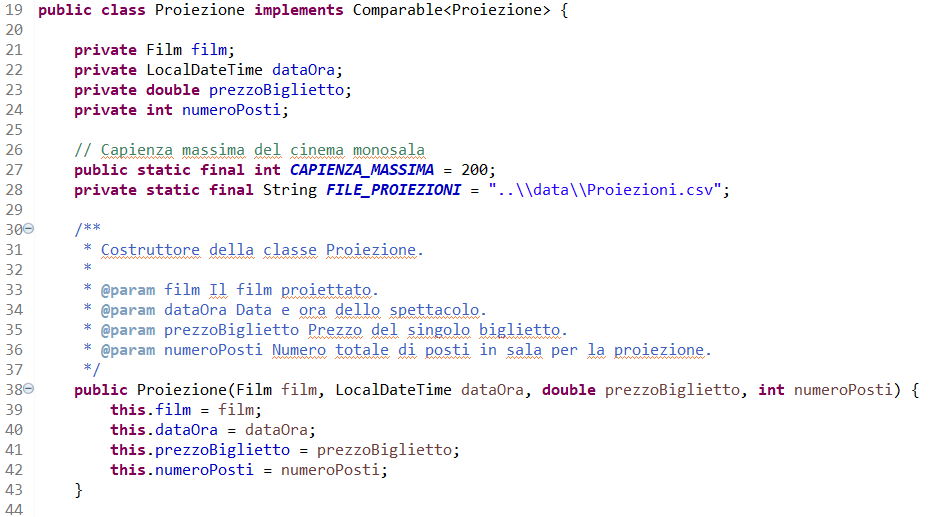
\includegraphics[scale=0.6]{IMGS/Proiezione}
\caption{I campi e il costruttore della classe Proiezione}
\end{figure}

\subsubsection{La classe Prenotazione}
La classe Prenotazione estende direttamente Object costruisce oggetti di tipo prenotazione usati nel menù utente della classe cliente, descritta in sezione \ref{subsubsec:Cliente}, contiene anche i metodi usati da quest'ultima per effettuare verifiche sulle stringhe inserite dall'utente e per interagire con il file prenotazioni.csv; questa classe fornisce inoltre i metodi per inserire, modificare o cancellare una prenotazione attraverso il menù utente; i campi di prenotazione sono:

\begin{center}
\begin{varwidth}{\textwidth}
\begin{itemize}
\item[•] \textbf{private String IDutente}
\item[•] \textbf{private String Nome} 
\item[•] \textbf{private String Cognome}
\item[•] \textbf{private LocalDateTime Proiezione\_ Data}
\item[•] \textbf{private String Proiezione\_ Titolo} 
\item[•] \textbf{private int ID\_ prenotazione}
\item[•] \textbf{private int numeroPosti}
\item[•]\textbf{private double Prezzo\_ Biglietto}
\end{itemize}
\end{varwidth}
\end{center}

che modellano rispettivamente l'ID univoco assegnato all'utente in fase di registrazione (si veda la sezione \ref{subsubsez:Registrarsi}), il nome e il cognome dell'utente, la data e l'orario della proiezione in formato AAAA-MM-GG HH:MM:SS, l'ID della prenotazione, che viene assegnata come intero in ordine crescente dal metodo public static int generaNuovoID(), il numero di posti prenotati e il prezzo del biglietto.
Questa classe contiene i metodi get e set per i suoi campi.

\subsubsection{La classe Guest}\label{subsubsec:Guest}

\subsubsection{La classe Cliente}\label{subsubsec:Cliente}

\subsubsection{La classe Proiezionista}\label{subsubsec:Proiezionista}

\subsubsection{La classe Bigliettaio}\label{subsubsec:Bigliettaio}

\subsubsection{La classe CineMaX}\label{subsubsec:CineMaX}
La classe CineMaX è la classe in cui si trova il metodo Main (che contiene il ciclo di esecuzione principale) e tutti i metodi necessari al login e alla registrazione di un account utente; tutti i metodi di questa classe a parte Main hanno visibilità private in quanto l'unica classe in cui devono essere utilizzati è questa (vengono usati all'interno del Main). Maggiori dettagli riguardo questa classe saranno forniti nella sezione\ref{sez:cicloprincipale} in cui si illustrano le funzionalità del ciclo di esecuzione principale dell'applicazione.


\subsection{Il ciclo di esecuzione principale}
Il metodo main contiene il ciclo di esecuzione principale dell'applicazione, che garantisce l'esecuzione fino a quando la variabile boolean On, inizializzata a true, non viene posta false nel logout. Prima di entrare nell'esecuzione il programma dichiara anche la variabile di tipo Guest loggeduser che sarà usata per il login dell'utente.

\label{sez:cicloprincipale}
Durante l'esecuzione dell'applicazione viene mostrato all'utente il menù principale mostrato in figura \ref{fig:menuprincipale}, che consente di navigare nel programma inserendo da tastiera il valore corrispondente alla funzionalità scelta dall'utente; ogni scelta possibile corrisponde al case di uno switch/case e ogni sottomenù è allo stesso modo uno switch/case che rimane in esecuzione fino a quando l'utente decide di ritornare al menù principale.

\begin{figure}[!htbp]
\centering
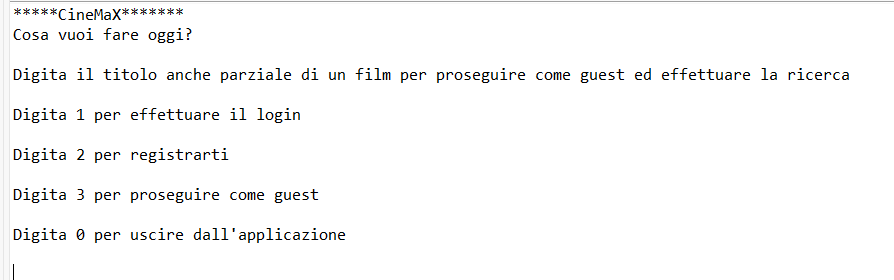
\includegraphics[scale=0.5]{IMGS/menuavvio}
\caption{Il menù principale}\label{fig:menuprincipale}
\end{figure}

Come si può vedere in figura \ref{fig:metodomain} il menù principale è costruito con System.out.println(String) e l'input da tastiera per mezzo dello Scanner(System.in) Kinput, il cui valore entra nello switch principale che lo confronta con una stringa.
\begin{figure}[!htbp]
\centering
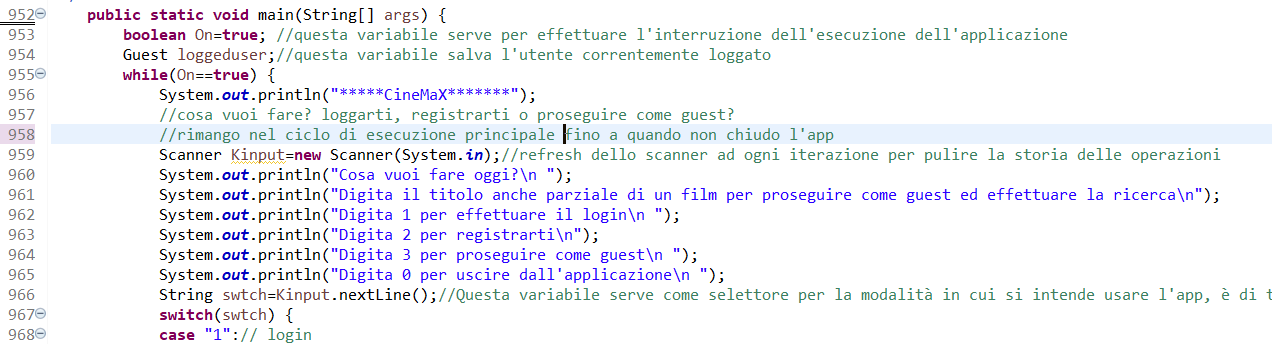
\includegraphics[scale=0.5]{IMGS/metodomain}
\caption{Il menù principale nel metodo main}\label{fig:metodomain}
\end{figure}

\subsubsection{Registrarsi}\label{subsubsez:Registrarsi}

\subsubsection{Effettuare il login}

\subsubsection{Login come Guest e ricerca di un film}
Se si digita un qualsiasi carattere che non corrisponde alle scelte possibili nel menù principale, si entra nel caso di default dello switch/case principale, che interpreta la stringa data in input dall'utente come il titolo (intero o parziale) di una proiezione ed effettua una ricerca nel palinsesto per mostrare tutte le proiezioni con quel nome disponibili. Per farlo l'utente deve essere loggato come guest quindi per prima cosa si procede a creare un nuovo oggetto di tipo guest e salvarlo nella variabile loggeduser, che sarà usata per invocare il metodo public void cercaProiezione() della classe Guest, che implementa l'interfaccia di ricerca di una proiezione. Dopo aver effettuato la ricerca si rimarrà quindi loggati come guest, quindi sarà possibileeffettuare una nuova ricerca, registrarsi con il metodo statico CineMax.Registrati()(si veda la sezione \ref{subsubsez:Registrarsi}) o tornare al menù principale. 
Questa modalità è uguale al caso 3 dello switch/case principale, che corrisponde all'accesso come guest per cui è solamente possibile registrarsi o effettuare la ricerca di una proiezione nel palinsesto.

\begin{figure}[!htbp]
\centering
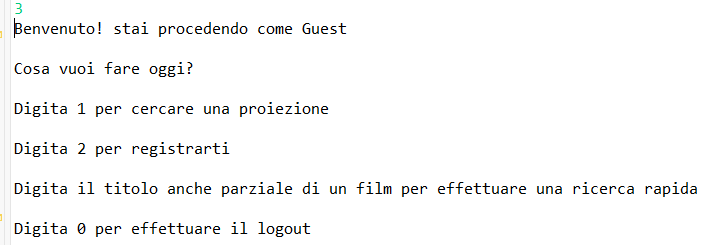
\includegraphics[scale=0.5]{IMGS/menuguest}
\caption{il menù dell'interfaccia guest}
\end{figure}

\begin{figure}[!htbp]
\centering
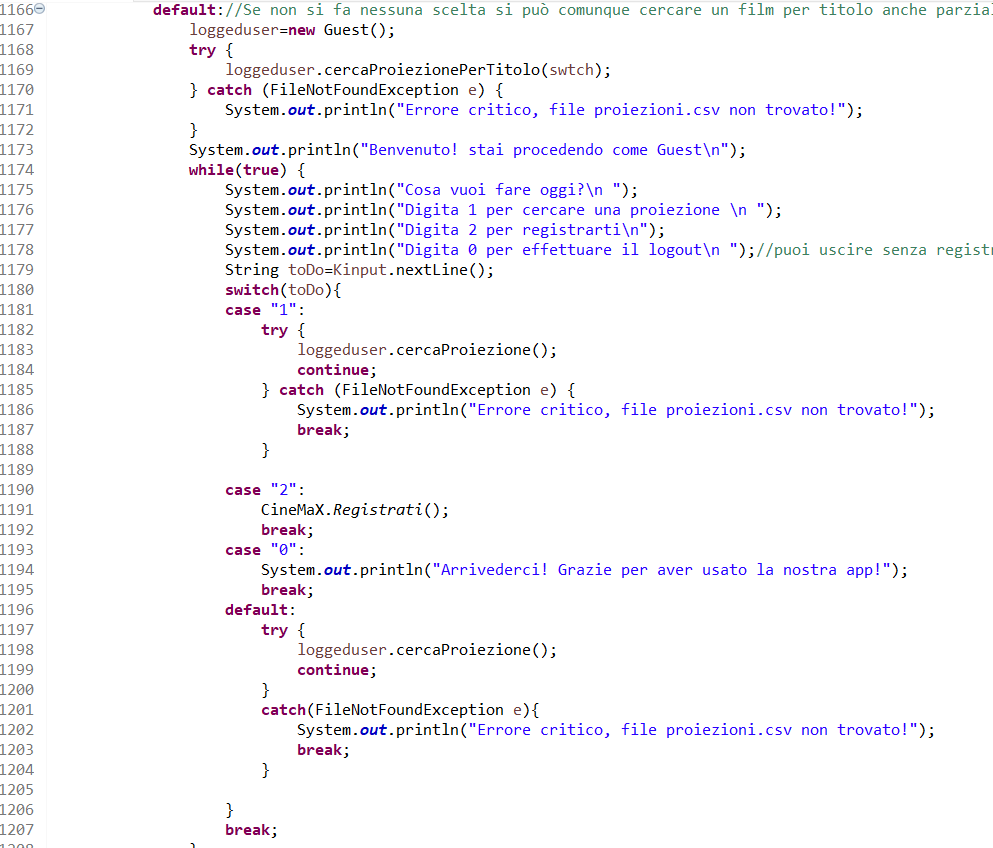
\includegraphics[scale=0.5]{IMGS/default}
\caption{Caso default e interfaccia guest}
\end{figure}

\subsubsection{Logout}
Quando si effettua il logout dall' applicazione, corrispondente all'input 0 da parte dell' utente nel menù principale, viene inizializzata la variabile boolean On a false ed eseguito un comando continue, in questo modo il codice salta alla successiva esecuzione del ciclo while (On=true)la cui condizione non sarà verificata e dunque il ciclo si arresterà, terminando l'applicazione; quando il ciclo di esecuzione principale termina viene mostrato a schermo un messaggio di arrivederci.

\begin{figure}[!htbp]
\centering
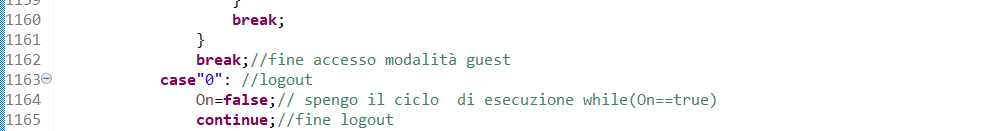
\includegraphics[scale=0.5]{IMGS/logout}
\caption{Logout}
\end{figure}

\subsection{Funzionalità dell'utente di tipo cliente}

\subsubsection{Ricerca di una proiezione}

\subsubsection{Effettuare una prenotazione}

\subsubsection{Cancellare una prenotazione}

\subsection{Funzionalità dell'utente di tipo proiezionista}

\subsubsection{Ricerca di una proiezione}

\subsubsection{Effettuare una prenotazione}

\subsubsection{Cancellare una prenotazione}

\subsection{Funzionalità dell'utente di tipo bigliettaio}

\subsubsection{Visualizzare tutte le prenotazioni in data odierna}

\subsubsection{Visualizzare le prenotazioni effettuate da un cliente}



\section{Data set di test}

\chapter{Limiti della soluzione proposta}

\chapter{Bibliografia}


\end{document}